%%%%%%%%%%%%%%%%%%%%%%%%%%%%%%%%%%%%%%%%%
% Short Sectioned Assignment LaTeX Template Version 1.0 (5/5/12)
% This template has been downloaded from: http://www.LaTeXTemplates.com
% Original author:  Frits Wenneker (http://www.howtotex.com)
% License: CC BY-NC-SA 3.0 (http://creativecommons.org/licenses/by-nc-sa/3.0/)
%%%%%%%%%%%%%%%%%%%%%%%%%%%%%%%%%%%%%%%%%

%----------------------------------------------------------------------------------------
%	PACKAGES AND OTHER DOCUMENT CONFIGURATIONS
%----------------------------------------------------------------------------------------

\documentclass[a4paper, 12pt]{report} % A4 paper and 11pt font size

% ---- Entrada y salida de texto -----

\usepackage[T1]{fontenc} % Use 8-bit encoding that has 256 glyphs
\usepackage[utf8]{inputenc}
\usepackage{ascii}
%\usepackage{fourier} % Use the Adobe Utopia font for the document - comment this line to return to the LaTeX default

% ---- Idioma --------

\usepackage[spanish, es-tabla]{babel} % Selecciona el español para palabras introducidas automáticamente, p.ej. "septiembre" en la fecha y especifica que se use la palabra Tabla en vez de Cuadro

% ---- Otros paquetes ----

\usepackage{amsmath,amsfonts,amsthm} % Math packages
%\usepackage{graphics,graphicx, floatrow} %para incluir imágenes y notas en las imágenes
\usepackage{graphics,graphicx, float} %para incluir imágenes y colocarlas
\usepackage{epstopdf} 
\usepackage[bookmarks = true, colorlinks=true, linkcolor = black, citecolor = magenta, menucolor = black, urlcolor = blue]{hyperref} 
\usepackage{url}
\usepackage{color}
\definecolor{gray97}{gray}{.97}
\definecolor{gray75}{gray}{.75}
\definecolor{gray45}{gray}{.45}

\usepackage{listings}
\lstset{ frame=Ltb,
	framerule=0pt,
	aboveskip=0.5cm,
	framextopmargin=3pt,
	framexbottommargin=3pt,
	framexleftmargin=0.4cm,
	framesep=0pt,
	rulesep=.4pt,
	backgroundcolor=\color{gray97},
	rulesepcolor=\color{black},
	%
	stringstyle=\ttfamily,
	showstringspaces = false,
	basicstyle=\small\ttfamily,
	commentstyle=\color{gray45},
	keywordstyle=\bfseries,
	%
	numbers=left,
	numbersep=15pt,
	numberstyle=\tiny,
	numberfirstline = false,
	breaklines=true,
}

% minimizar fragmentado de listados
\lstnewenvironment{listing}[1][]
{\lstset{#1}\pagebreak[0]}{\pagebreak[0]}

\lstdefinestyle{consola}
{basicstyle=\scriptsize\bf\ttfamily,
	backgroundcolor=\color{gray75},
}

\lstdefinestyle{C}
{language=C,
}

\usepackage{parskip}

% Para hacer tablas comlejas
%\usepackage{multirow}
%\usepackage{threeparttable}

%\usepackage{sectsty} % Allows customizing section commands
%\allsectionsfont{\centering \normalfont\scshape} % Make all sections centered, the default font and small caps

\usepackage{fancyhdr} % Custom headers and footers
\pagestyle{fancyplain} % Makes all pages in the document conform to the custom headers and footers
\fancyhead{} % No page header - if you want one, create it in the same way as the footers below
\fancyfoot[L]{} % Empty left footer
\fancyfoot[C]{} % Empty center footer
\fancyfoot[R]{\thepage} % Page numbering for right footer
\renewcommand{\headrulewidth}{0pt} % Remove header underlines
\renewcommand{\footrulewidth}{0pt} % Remove footer underlines
\setlength{\headheight}{13.6pt} % Customize the height of the header

\numberwithin{equation}{section} % Number equations within sections (i.e. 1.1, 1.2, 2.1, 2.2 instead of 1, 2, 3, 4)
\numberwithin{figure}{section} % Number figures within sections (i.e. 1.1, 1.2, 2.1, 2.2 instead of 1, 2, 3, 4)
\numberwithin{table}{section} % Number tables within sections (i.e. 1.1, 1.2, 2.1, 2.2 instead of 1, 2, 3, 4)

\setlength\parindent{0pt} % Remov%Para conseguir que en las páginas en blanco no ponga cabecerass

\makeatletter
\def\clearpage{%
  \ifvmode
    \ifnum \@dbltopnum =\m@ne
      \ifdim \pagetotal <\topskip
        \hbox{}
      \fi
    \fi
  \fi
  \newpage
  \thispagestyle{empty}
  \write\m@ne{}
  \vbox{}
  \penalty -\@Mi
}
%\makeatotheres all indentation from paragraphs - comment this line for an assignment with lots of text

\makeatletter

\newcommand\frontmatter{%
    \cleardoublepage
  %\@mainmatterfalse
  \pagenumbering{roman}}

\newcommand\mainmatter{%
    \cleardoublepage
 % \@mainmattertrue
  \pagenumbering{arabic}}

\newcommand\backmatter{%
  \if@openright
    \cleardoublepage
  \else
    \clearpage
  \fi
 % \@mainmatterfalse
   }

\makeatother

\usepackage{titlesec}
\titleformat{\chapter}[display]   
{\normalfont\huge\bfseries}{\chaptertitlename\ \thechapter}{20pt}{\Huge}   
\titlespacing*{\chapter}{0pt}{-50pt}{40pt}

\usepackage{geometry}% http://ctan.org/pkg/geometry
\newcommand{\mygeometry}[1]{%
  \geometry{right=#1,left=\dimexpr#1\relax}% Set new geometry
}
\mygeometry{30mm}% 25mm left/right margins

\newcommand{\horrule}[1]{\rule{\linewidth}{#1}} % Create horizontal rule command with 1 argument of height

%----------------------------------------------------------------------------------------
%	TÍTULO Y DATOS DEL ALUMNO
%----------------------------------------------------------------------------------------
\begin{document}

\begin{titlepage}
 
 
\newlength{\centeroffset}
\setlength{\centeroffset}{-0.5\oddsidemargin}
\addtolength{\centeroffset}{0.5\evensidemargin}
\thispagestyle{empty}

\noindent\hspace*{\centeroffset}
\begin{minipage}{\textwidth}

\centering

\includegraphics[width=0.9\textwidth]{imagenes/logo_ugr.jpg}\\[1.4cm]

\textsc{ \Large TRABAJO FIN DE GRADO\\[0.2cm]}
\textsc{ INGENIERÍA INFORMÁTICA}\\[1cm]
% Upper part of the page
% 
% Title
{\Huge\bfseries Desarrollo de un Sistema Experto de Análisis Musical\\
}
\noindent\rule[-1ex]{\textwidth}{3pt}\\[3.5ex]
{\large\bfseries }
\end{minipage}

\vspace{2.5cm}
\noindent\hspace*{\centeroffset}
\begin{minipage}{\textwidth}
\centering

\textbf{Autor}\\ {Laura Olga Tirado López}\\[2.5ex]
\textbf{Directores}\\
{Juan Luis Castro Peña}\\[2.5ex]

\includegraphics[width=0.3\textwidth]{imagenes/etsiit_logo.png}\\[0.1cm]
\textsc{Escuela Técnica Superior de Ingenierías Informática y de Telecomunicación}\\
\textsc{---}\\
Granada, Junio de 2017
\end{minipage}
%\addtolength{\textwidth}{\centeroffset}
%\vspace{\stretch{2}}
\end{titlepage}

%----------------------------------------------------------------------------------------
% DOCUMENTO
%----------------------------------------------------------------------------------------

\newpage

%----------------------------------------------------------------------------------------
%	Prefacio
%----------------------------------------------------------------------------------------

\frontmatter

\thispagestyle{empty}

\begin{center}
{\large\bfseries Desarrollo de un Sistema Experto de Análisis Musical}\\
\end{center}
\begin{center}
Laura Olga Tirado López\\
\end{center}

%\vspace{0.7cm}
\noindent{\textbf{Palabras clave}: sistema, experto, análisis, analizar, música, musical, coro, coral, quintas, octavas, armonía, armónico, melodía, melódico, contrapunto, voces, partitura}\\

\vspace{0.7cm}
\noindent{\textbf{Resumen}}\\

Se pretende desarrollar una aplicación basada en reglas para poder analizar \textit{corales} o partituras de coro.

\bigskip

El objetivo es implementar un sistema experto que permita a los usuarios analizar partituras de coro a cuatro voces para su posterior corrección, pudiendo así mejorarlas tanto a nivel armónico como a nivel melódico y de contrapunto.

\bigskip

El sistema se basará en conocimiento experto sobre lenguaje musical, composición y armonía clásica proporcionado por varios profesores de armonía y composición del Conservatorio Profesional Ángel Barrios, músicos titulados y otras fuentes tales como libros y tratados. 

\bigskip

Las funcionalidades que proporcionará este sistema se dividirán en dos clases:

\begin{itemize}
	\item \textbf{Análisis armónico}: consistente en la búsqueda de errores que comprendan, al menos dos de las voces, tales como acordes incompletos, secuencias armónicas incorrectas y búsqueda de disonancias.
	\item  \textbf{Análisis melódico}: consistente en la búsqueda de errores referidos a las melodías de las voces, tales como conducción incorrecta de las mismas, falta de coherencia y saltos o movimientos disonantes. 
\end{itemize}

\bigskip

El interés principal de este proyecto es poder desarrollar una herramienta para compositores o estudiantes de composición que haga una función análoga a la de un corrector ortográfico y gramatical de un editor de textos, aplicada a la composición y edición de partituras.

\cleardoublepage


\thispagestyle{empty}


\begin{center}
{\large\bfseries Development of an Expert System for Musical Analysis}\\
\end{center}
\begin{center}
Laura Olga Tirado López\\
\end{center}

%\vspace{0.7cm}
\noindent{\textbf{Keywords}: system, expert, analysis, analize, music, musical, choir, fifths, eights, harmony, harmonic, melody, melodic, voices, sheet, counterpoint}\\

\vspace{0.7cm}
\noindent{\textbf{Abstract}}\\

My intention is develop an app that implements an expert system to analysis \textit{choir} sheets.

\bigskip

This development aims to create a rule bases engine that allows users analize choir sheet musics for later correction, being able to improve their harmonies, melodies and counterpoint.

\bigskip

The system will be based on expert knwoledge about music notation, composing and classic harmony provided by many harmony and composition teachers of Conservatorio Profesional Ángel Barrios, musicians and another sources such as books and musical tratrises.

\bigskip

Features provided by this system will be of two grades:

\begin{itemize}
	\item \textbf{Harmonic analysis}: consisting on search for errors involving, at least, two of the voices, such as incomplete chords, incorrect harmonic sequences and  dissonances.
	\item  \textbf{Melodic analysis}: consisting on search for errors involving melodies, such as incorrect voice guidance, lack of coherence and dissonant movements. 
\end{itemize}

\bigskip

The main interest of this project is being able of develop a tool for composers or music students that performs a function analogous to an spelling and grammar checker, applied to composing and writing music. 

\newpage
\thispagestyle{empty}

\noindent\rule[-1ex]{\textwidth}{2pt}\\[4.5ex]

D. \textbf{Juan Luis Castro Peña}, Profesor del Área de XXXX del Departamento de Ciencias de la Computación e Inteligencia Artificial de la Universidad de Granada.

\vspace{0.5cm}

\textbf{Informa:}

\vspace{0.5cm}

Que el presente trabajo, titulado \textit{\textbf{Desarrollo de un Sistema Experto de Análisis Musical}},
ha sido realizado bajo su supervisión por \textbf{Laura Olga Tirado López}, y autorizamos la defensa de dicho trabajo ante el tribunal que corresponda.

\vspace{0.5cm}

Y para que conste, expiden y firman el presente informe en Granada a X de mes de 2017.

\vspace{1cm}

\textbf{El director:}

\vspace{5cm}

\noindent \textbf{Juan Luis Castro Peña}

\chapter*{Agradecimientos}
\thispagestyle{empty}

       \vspace{1cm}

\bigskip
A mi familia, por apoyarme y hacer posible que esté donde estoy hoy.

\bigskip
A mis amigos, por estar siempre ahí y animarme a seguir cuando las cosas se tuercen.

\bigskip
A mis compañeros de informátoca, porque sin ellos esta etapa que es la vida universitaria no habría tenido tantas risas.

\bigskip
A mis compañeros de la DEIIT, siempre dispuestos a escuchar mis quejas y ayudarme con mis problemas.

%----------------------------------------------------------------------------------------
%	Índices
%----------------------------------------------------------------------------------------

\newpage %inserta un salto de página

\tableofcontents % para generar el índice de contenidos

\listoffigures

\listoftables

\newpage

%----------------------------------------------------------------------------------------
%	Capítulos
%----------------------------------------------------------------------------------------


\mainmatter
\chapter*{Introducción}
\addcontentsline{toc}{chapter}{Introducción}

La música es un arte que ha acompañado al ser humano desde casi sus inicios. Ésta se ha ido desarrollando a lo largo de los siglos, adaptándose a la época y sus avances, creando nuevos instrumentos y nuevos estilos. Con la evolución de los distintos estilos musicales se fue desarrollando de igual manera la notación musical, desde las primeras notaciones creadas por la cultura griega, a base de letras del alfabeto y algunos símbolos como puntos, hasta la notación abstracta utilizada hoy en día. 

En la actualidad, gracias a las nuevas tecnologías, disponemos de editores de partituras que realizan la misma función que los editores de texto que encontramos en cualquier ordenador: poder crear y editar una partitura. Sin embargo, una de las funcionalidades que ofrecen los editores de texto y también los móviles son los correctores ortográficos y/o gramaticales, los cuáles en los dispositivos como smartphones y tablets son ampliamente utilizados. 

Algunos editores de partituras, como \textit{Sibelius}, en sus últimas versiones sí añaden parte de esta funcionalidad, pudiendo buscar algunos tipos de errores en partituras, tales como quintas u octavas directas. Sin embargo, las reglas de armonía clásica en las que se basan la mayoría de composiciones, salvo las basadas en nuevas corrientes musicales como música contemporánea o experimental, exponen una gran cantidad de restricciones sobre cómo debe componerse una pieza musical de estilo clásico para que sea correcta y coherente.  Estas reglas tratan desde la correcta disposición de las notas de un acorde hasta la conducción de melodías y la búsqueda de sonoridades consonantes, evitando las disonancias o utilizándolas de maneras determinadas para conseguir efectos sonoros específicos. 

El interés de este proyecto radica pues en la falta de una herramienta de este tipo que permita a compositores y estudiantes de composición y armonía poder corregir errores en sus composiciones o ejercicios de forma automática, con el objetivo de mejorarlas.

Dado que la música abarca una gran variedad de estilos y formas musicales, he decidido para este proyecto centrarme en una de las más extendidas y utilizadas dado su interés para la enseñanza de este campo: los corales o partituras de coro. Esta forma musical proporciona el entorno perfecto para poder estudiar las reglas armónicas, melódicas y de contrapunto al tener cuatro melodías cantadas por cuatro voces independientes que se van entrelazando a lo largo de la obra. 

La realización de este proyecto se centra en la resolución de un problema muy concreto con un entorno muy específico. Además, aunque hay reglas de armonía que son completamente indiscutibles, existen gran cantidad de excepciones a éstas y cierta subjetividad; algo puede no estar necesariamente mal pero no llegar a ser del todo correcto. Un caso sería la conducción melódica de las voces, la cual puede hacerse de diversas maneras según lo que quiera transmitir el compositor en un momento determinado.

Por estos motivos, mi propuesta para poder implementar esta funcionalidad se basa en un sistema experto, el cual a partir de una base de conocimiento de teoría musical y reglas armónicas pueda analizar las partituras de igual manera que un experto en esta materia, teniendo en cuenta la posible subjetividad del análisis.

En los siguientes capítulos se explicará detalladamente el proceso de desarrollo de este sistema, así como los resultados obtenidos tras su implementación. Además, ara facilitar la comprensión de este trabajo, los términos y definiciones musicales que aparecen a lo largo del documento pueden ser consultados en el \hyperref[glosario]{\textbf{Anexo}}.


\chapter*{1. Especificación de requisitos}
\addcontentsline{toc}{chapter}{1. Especificación de requisitos}

La espeficićación de requisitos de un sistema experto comprende la determinación de requerimientos de información, funcionales y de entrada de datos. En esta fase del desarrollo debemos determinar qué datos de entrada, proporcionados por el usuario, necesita el sistema para funcionar, las operaciones que llevará a cabo sobre dichos datos y los resultados que espera el usuario obtener del sistema.  

Para poder realizar esta fase del desarrollo, necesitamos extraer esta serie de requisitos de los que serán los usuarios finales del sistema.

Como se menciona en la introducción, este sistema está dirigido a compositores o estudiantes de composición y armonía que desean mejorar sus obras o comprobar si éstas no contienen errores armónicos y/o melódicos. Estos serían nuestros usuarios finales y a los que he consultado qué respuesta esperarían del sistema, es decir, que información debería analizarse en la partitura y cómo mostrar los posibles errores encontrados, así como qué información sería necesaria proporcionar para poder llevar a cabo el análisis deseado. 

\section*{1.1 Requisitos de información}
\addcontentsline{toc}{section}{1.1 Requisitos de información}


El sistema, una vez finalizado el análisis, mostrará una lista seriada de los diferentes errores y faltas encontrados. Éstos estarán debidamente explicados y señalizados en la partitura, indicando las voces implicadas y el compás en el que aparecen. 

Dado que estos errores pueden ser de origen diverso, armónico o melódico, se crearán listados específicos para cada tipo de análisis, a fin de facilitar el entendimiento de los resultados y la experiencia del usuario.   

\section*{1.2 Requisitos funcionales}
\addcontentsline{toc}{section}{1.2 Requisitos funcionales}


El eje principal de este sistema radica en dos funciones principales: análisis armónico y análisis melódico.

La realización del análisis armónico implica la comprobación de los siguientes hechos:

\begin{itemize}

	\item Quintas paralelas: dadas dos voces, éstas no pueden producir dos intervalos de quinta consecutivos. No obstante si el segundo intervalo de quinta es de tipo aumentado o disminuido y no se encuentra en voces extremas no se considerará falta.

	\item Quintas directas: dadas dos voces, éstas no pueden producir un intervalo de quinta por movimiento directo.

	\item Octavas paralelas: dadas dos voces, éstas no pueden producir dos intervalos de octava consecutivos. 

	\item Octavas directas: dadas dos voces, éstas no pueden producir un intervalo de octava por movimiento directo.

	\item Tritono: dadas dos voces, éstas no pueden producir un intervalo de cuarta aumentada o tritono. No obstante si éste viene preparado por movimiento conjunto u oblicuo de las voces no se considerará falta.

	\item Duplicación de sensible: en ningún caso se podrá duplicar la sensible de la tonalidad. 

	\item Búsqueda de acordes incompletos: todos los acordes deberán de tener la fundamental, la tercera y la quinta del acorde en al menos una voz, especialmente si están invertidos. No obstante, se puede dar la situación de que el acorde de tónica quede incompleto, con la ausencia de la quinta, en la cadencia.

	\item Segunda inverión consecutiva: en ningún caso podrá haber dos acordes en segunda inversión consecutivos.

	\item Lógica tonal: la armonía de la obra deberá seguir, en la medida de lo posible, el esquema indicado en la figura .

		\begin{itemize}

			\item La tónica o primer grado (I) podrá moverse hacia cualquier otro grado de la escala.
			\item La supertónica o segundo grado (II) podrá moverse hacia la tónica, cuarto, quinto o séptimo grado.
			\item La mediante, modal o tercer grado (III) podrá moverse hacia sexto grado.
			\item La subdominante o cuarto grado (IV) podrá moverse hacia el primer, segundo, quinto o séptimo grado.
			\item La dominante o quinto grado (V) podrá moverse hacia el primer, sexto o séptimo grado.
			\item La superdominante o sexto grado (VI) podrá moverse hacia el segundo o cuarto grado.
			\item La subtónica o séptimo grado (VII podrá moverse hacia el primer, tercer o quinto grado.
		\end{itemize}

		Por otra parte, no podrán darse en ningún caso las siguientes sucesiones de acordes:

		\begin{itemize}
			\item I-II en estado fundamental.
			\item II-III en estado fundamental,
			\item III-IV en estado fundamental.
		\end{itemize}

\end{itemize}

La realización del análisis melódico implica la comprobación de los siguientes hechos:

\begin{itemize}

	\item Resolución de sensibles: la sensible de la tonalidad deberá resolver siempre en la tónica.

	\item Resolución de séptimas: la séptima de dominante deberá resolver siempre por movimiento por grado conjunto descendente y deberá estar preparada.

	\item Segunda aumentada: en ningún caso podrá haber un intervalo de segunda aumentada entre dos notas consecutivas en una misma voz.

	\item Tritono melódico: en ningún caso podrá haber un intervalo de cuarta aumentada o tritono entre dos notas consecutivas en una misma voz.

	\item Contrapunto en voces extremas: deberá predominar el movimiento contrario en las voces extremas sobre el movimiento oblicuo y, especialmente, directo.

	\item Contrapunto del salto: si hay dos movimientos (saltos) en la misma dirección, ascendente o descendente, la primera y la última nota no pueden ser disonantes.

	\item Melodía incoherente: deberá predominar el movimiento por grados conjuntos en las melodías, evitando hacer demasiados saltos.

\end{itemize}


\section*{1.3 Requisitos de entrada de datos}
\addcontentsline{toc}{section}{1.3 Requisitos de entrada de datos}


Los datos de entrada necesarios para el funcionamiento del sistema son las opciones de los distintos tipos de análisis posibles y la partitura en la que se van a realizar. 
\chapter*{2. Adquisión de conocimiento}
\addcontentsline{toc}{chapter}{2. Adquisión de conocimiento}

La adquisición y educción del conocimiento constituye una de las fases más importantes del desarrollo de este tipo de sistemas. En esta etapa es donde el Ingeniero del Conocimiento interactúa con el experto para obtener la información sobre la solución de los problemas, así como las estrategias utilizadas para la obtención de cada solución. Además de consultar con el experto, también se adquiere conocimiento de otras fuentes como libros, tratados, estudios, etc. Este proceso supone el ``cuello de botella'' del desarrollo.

Para este proyecto, el conocimiento ha sido adquirido a partir de entrevistas con varios músicos y de diversos tratados, libros y apuntes proporcionados por profesorado del Conservatorio Profesional Ángel Barrios de Granada.

\section*{2.1 Entrevistas con los expertos}
\addcontentsline{toc}{section}{2.1 Entrevistas con los expertos}



%\input{capitulos/03_Analisis}
%\input{capitulos/04_Diseno}
%\chapter{Implementación}

La implementación de este proyecto se ha llevado a cabo en dos fases diferenciadas: la creación del sistema experto y el desarrollo de la aplicación web,utilizada como interfaz, en la que será embebido. 

Todo el código puede ser consultado en \cite{CODIGO}.

\section{Sistema experto}

El primer paso fue la creación de un prototipo utilizando el entorno de CLIPS. A continuación, se explican las decisiones tomadas a lo largo del desarrollo de este prototipo.

\subsection{Formato de los datos de entrada: partitura}

Una de las primeras cuestiones fue cómo obtener la información necesaria del XML en el que está contenida la partitura. Dado que CLIPS no puede procesar el XML para leer el contenido de las etiquetas, está funcionalidad tenía que ser realizada por Python. Sin embargo, definimos las estructuras que debían tener los ficheros para poder ser leídos por CLIPS y añadir esa información en forma de hechos.

Los datos que teníamos que extraer de la partitura eran:

\begin{itemize}

	\item La \textbf{tonalidad} de la obra. La tonalidad es la que nos define la \textit{escala musical} sobre la que está construido el coral. Nos da la relación entre los acordes y sus funciones tonales. La tonalidad está compuesta por el nombre y el modo.

	\item El \textbf{compás}. El compás nos indica cuántas figuras de un determinado tipo hay en cada pulso. El compás está compuesto por dos números que nos indican el número de pulsos y el tipo de figura que dura un pulso:

	\begin{itemize}
		\item 1: redonda
		\item 2: blanca
		\item 4: negra
		\item 8: corchea
	\end{itemize}

	\item Las \textbf{notas} de cada voz. Las notas musicales vienen definidas por su nombre, su altura, su duración y su alteración.

	\item Los \textbf{movimientos} de cada voz. Los movimientos nos indican si la voz, de una nota a otra, se mueve de forma ascendente, descendente o se mantiene.

\end{itemize}

Para cada uno de estos datos se creo una plantilla con la instrucción ``\texttt{deftemplate}'', al igual que para el resto de hechos como se mencionó en el capítulo \textit{Adquisición de conocimientos}. 

\subsubsection{Estructura del archivo de notas}

Una de las mayores dificultades fue decidir la estructura del archivo que contendría la información sobre las notas. Cada nota tiene una duración independiente, lo cual a la hora de realizar el análisis armónico resulta muy complejo. Al analizar la armonía de una obra tenemos que tener en cuenta todas las voces al mismo tiempo, analizamos de forma vertical. Sin embargo, en una misma parte cada nota de cada voz puede tener una duración distinta y por ende puede formarse más de un acorde en dicha parte. Esto significa que no siempre va a haber el mismo número de acordes, ni de notas, en cada compás.

En la práctica, a un experto este hecho no le resulta un problema, porque puede observar las voces gráficamente y poder determinar cuándo termina la duración de cada nota y el acorde. En cambio, para un sistema experto, al no saber dónde termina cada nota con respecto a las demás, no puede hacer esas deducciones de manera tan sencilla. 

Para solucionar este problema, decidí subdividir todas las notas de todas las voces a semicorcheas, que es la figura musical más pequeña que se suele utilizar en los corales. De esta forma, conseguimos que en todos los compases haya el mismo número de notas en cada voz.

En la siguiente figura, se muestra gráficamente lo que supone esta transformación:


\begin{figure}[H]
	\centering
	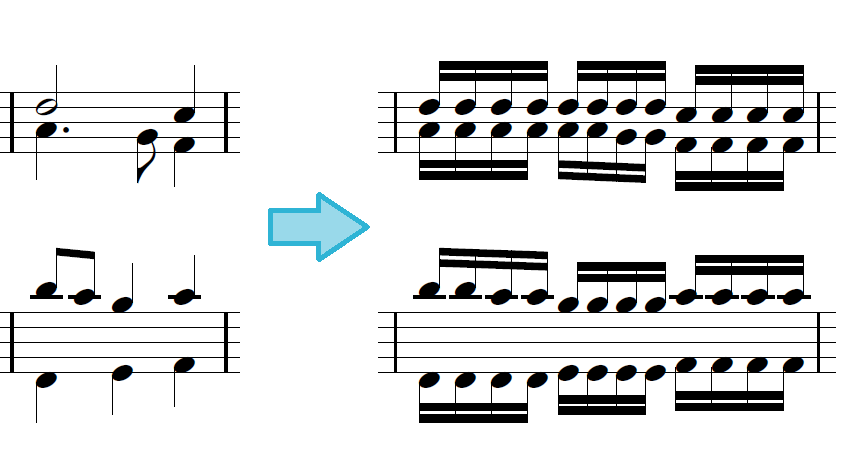
\includegraphics[scale=0.5]{imagenes/division.png}
	\caption{Subdivisión de un compás del coral ``Aus meines Herzens Grunde'' de \textit{J.S.Bach} a semicorcheas}
	\label{fig5.1.1}
\end{figure}

Como podemos ver, al realizar esta subdivisión podemos ir analizando en bloques equivalente en tiempo. Los resultados del análisis no se ven afectados, dado que únicamente hemos modificado la duración de las notas, la cual no interviene en los errores que vamos a detectar.

En el caso del análisis melódico, no es necesario hacer esta subdivisión porque analizamos cada voz de manera independientede de las otras, analizamos la partitura horizontalmente.

\subsubsection{Formatos finales}

Las estructuras de los ficheros que leería el sistema experto quedarían de la siguiente manera:

\begin{itemize}

	\item Fichero de la tonalidad:

		\begin{lstlisting}[frame=single]

			Nombre Modo

		\end{lstlisting}

		Ejemplo:

		\begin{lstlisting}[frame=single]

			D Mayor

		\end{lstlisting} 

	\bigskip
	\item Fichero del compás:

		\begin{lstlisting}[frame=single]

			Partes Figura

		\end{lstlisting}

		Ejemplo:

		\begin{lstlisting}[frame=single]

			3 4

		\end{lstlisting} 

	\bigskip
	\item Fichero de notas: se crearía un fichero para cada voz.
	
		\begin{lstlisting}[frame=single]

			Nombre Alteracion Altura Nombre Alteracion Altura ...

		\end{lstlisting} 

		Ejemplo:

		\begin{lstlisting}[frame=single]

			A b 4 B 2 D s 3

		\end{lstlisting} 

	\bigskip
	\item Movimientos:

		\begin{lstlisting}[frame=single]

			Movimiento1 Movimiento2 Movimiento3 ...

		\end{lstlisting} 

		Ejemplo:

		\begin{lstlisting}[frame=single]

			Ascendente Ascendente Descendente

		\end{lstlisting} 

\end{itemize}

Los nombres de las notas se representarán con el cifrado americano, el empleado en el archivo XML. La equivalencia entre el cifrado americano y el empleado en occidente es:

\begin{itemize}

	\item Do $\rightarrow$ C
	\item Re $\rightarrow$ D
	\item Mi $\rightarrow$ E
	\item Fa $\rightarrow$ F
	\item Sol $\rightarrow$ G
	\item La $\rightarrow$ A
	\item Si $\rightarrow$ B

\end{itemize}

\subsection{Implementación del primer prototipo}

En el primer prototipo, no se modularizaron los hechos y reglas en función de los módulos descritos en los capítulos anteriores. Esto es porque aún no estaban definidas del todo las dependencias de las reglas respecto a los hechos ni la división del análisis armónico en dos partes realmente diferenciadas. 

Aunque en el análisis y el diseño quedan claras estas divisiones, a la hora de implementar las reglas, iban surgiendo muchas relaciones entre todos los hechos de la base de conocimiento. Por ejemplo, se esperaba que los hechos referidos a los movimientos de las voces únicamente fueran utilizados por el módulo del análisis melódico. Sin embargo, también es necesario para localizar algunos errores armónicos. Además, la existencia de algunos errores melódicos provoca a su vez errores armónicos y viceversa. 

Una vez se terminaron de implementar todas las reglas y hechos, se procedió a verificar y validar el prototipo. 

La  \textbf{verificación} consistió en comprobar que los ficheros se leían correctamente y los hechos deducidos se asertaban en el sistema de la manera esperada. Esto se comprobó fácilmente observando la ventana de hechos que aparece en la propia interfaz de CLIPS.

La \textbf{validación} se realizó creando archivos de prueba, con los formatos descritos anteriormente, que contuviesen al menos un error de cada tipo. Los modelos de prueba fueron recogidos de las fuentes bibliográficas, las cuáles contienen una gran cantidad de ejemplos

\subsection{Modularización del sistema}

Tras la creación del primer prototipo y su verificación y validación, comencé el proceso de modularización del sistema. 

Al estar implementadas todas las reglas y funcionalidades del sistema, este proceso, aunque tedioso, fue el más sencillo. 

Fui comprobando para cada regla los antencendentes que debían cumplirse y así poder agruparlas según los hechos que necesitaban.
Una vez agrupadas, pude definir los hechos asertados necesarios para cada uno de los módulos.

Como resultado final, obtuve los tres módulos de análisis, cada uno con sus reglas y hechos diferenciados. 

\section{Aplicación web}

La implementación de la aplicación web, como se comentó en el capítulo anterior, se ha hecho utilizando el framework DJango de Python.

La finalidad de implementar esta aplicación es proporcionar al sistema experto una interfaz agradable y sencilla de utilizar para el usuario. 

Este portal se encargará de las siguientes funciones:
\begin{itemize} 
	\item El envío de un formulario con las opciones de análisis seleccionadas por el usuario y el archivo de la partitura a analizar.
	\item La extracción de datos del archivo XML de la partitura y escritura de los mismos en ficheros según se describe en la sección anterior.
	\item La ejecución de los módulos seleccionados del sistema experto.
	\item Mostrar los errores detectados.
\end{itemize}

\subsection{Tratamiento del archivo XML}

Como se ha comentado antes, CLIPS no puede extraer la información de las etiquetas del archivo XML. Esta tarea es implementada por Python haciendo uso de la API \textit{ElementTree XML}. Esta API nos permite buscar etiquetas y leer el contenido de las mismas. 

Los archivos XML que contienen partituras, hacen uso de una gran cantidad de etiquetas. En este caso, para extraer los datos necesarios consultamos las siguientes:

\begin{itemize}

	\item \textit{Key}: para extraer la tonalidad.
	\item \textit{Time}: para extraer el compás.
	\item \textit{Note}: para extraer información de la nota. Dentro de ésta consultamos la siguientes subetiquetas:
		\begin{itemize}
			\item \textit{Pitch}: para extraer el nombre y la octava. 
			\item \textit{Accidental}: para comprobar si tenía una alteración accidental.
			\item \textit{Type} y \textit{Dot}: para extraer la duración.
			\item \textit{Voice}: para extraer la voz que canta dicha nota.
		\end{itemize}
\end{itemize}

La información contenida en las etiquetas se escribe en ficheros de acuerdo al formato que definimos.

\subsubsection{Determinación de movimientos melódicos}

Para el análisis melódico y algunas cuestiones del análisis armónico es necesario conocer la dirección que van tomando las melodías. Esta información no viene representada de forma explícita en el archivo de la partitura, sino que debemos de extraerla nosotros. 

Una vez se han creado los archivos que contienen las notas de las voces, vamos comprobando las notas dos a dos para determinar si la melodía hace un movimiento descendente, ascendente o se mantiene. 

La lista de movimientos de cada voz se escribe en un fichero para ser utilizado por los módulos de análisis.

\subsection{Integración del sistema experto}

Esta fase de la implementación fue la que presentó más problemas. Para integrar el sistema con la interfaz web he utilizado la librería PyCLIPS. Esta librería permite utilizar las funciones de CLIPS para crear sistema expertos en Python. Además, también permite cargar archivos creados en CLIPS y ejecutarlos.

Gracias a esta última característica, en un principio se pensó que únicamente sería necesario cargar los archivos de los módulos y  ejecutarlos cuando fuera necesario. Sin embargo, hubo que hacer algunas modificaciones.

El primer problema con el que me encontré fue que los archivos no podían cargarse. Tras buscar en la documentación de PyCLIPS \cite{PYCLIPS}, encontré la respuesta a este problema. PyCLIPS permite cargar archivos de CLIPS que contengan reglas o hechos, pero no ambas en un mismo fichero. Así pues, dividí los ficheros en ficheros con reglas y ficheros con hechos. 

De nuevo, surgió otro problema, esta vez con los archivos de hechos. En este caso, no se aceptaban las definiciones de las estructuras \texttt{deftemplate}. Para solucionarlo, decidí añadirlas utilizando explícitamente las funciones de PyCLIPS. A pesar de que parecía haberse solucionado, esto derivó en nuevos problemas asociados a dos funciones de CLIPS: las funciones \texttt{clear} y \texttt{reset}.

\bigskip
La función \texttt{clear} borra todo el entorno de CLIPS, eliminando de la memoria de trabajo todos los hechos, reglas, plantillas y funciones que estuviesen definidos.

\bigskip
La función \texttt{reset} reinicia el entorno, eliminando sólo los hechos y dejando en la memoria de trabajo todas las reglas, plantillas y funciones.

\bigskip

Antes de la ejecución de cada módulo se siguen los siguientes pasos:

\begin{itemize}
	\item Se transforma el XML a los archivos de entrada del sistema experto.
	\item Se limpia el entorno.
	\item Se reinicia el entorno.
	\item Se cargan las plantillas del módulo.
	\item Se cargan los hechos del módulo.
	\item Se cargan las reglas del módulo.
\end{itemize}

Debido a algún problema con la librería PyCLIPS o el intérprete de Python, la función \texttt{clear} no puede ejecutarse. Esto provoca que cada vez que se lancen los módulos del sistema, se redefinan las plantillas con las funciones de PyCLIPS. CLIPS no permite sobreescribir hechos o plantillas, por lo que nos daba un error de redefinición. 

Para el correcto funcionamiento del sistema, las plantillas debían ser definidas una única vez al inicio del sistema. Tras consultar la documentación y el foro de la comunidad encontré la solución: había que definir las plantillas en el archivo \texttt{urls.py}. Este archivo contiene las expresiones regulares de las ``urls'' en las que se visualizarán las secciones de la pagina web. Éste código se ejecuta una única vez al inicio de la aplicación, lo que nos permite evitar que las plantillas se creen una y otra vez.

Aunque se solucionó el problema de las plantillas, no se podía leer el archivo de hechos. Para asertar conjuntos de hechos en el entorno de CLIPS se utiliza la instrucción \texttt{deffacts}. Esta instrucción no era reconocida por la función \texttt{LoadFacts} de PyCLIPS, que es la encargada de cargar el archivo. Intenté modificar la sintaxis del archivo utilizando otras instrucciones como \texttt{assert}, que ``aserta'' los hechos en la memoria de trabajo, o escribiendo directamente los hechos, sin éxito. Al igual que con la función \texttt{clear}, no conseguía hacer que la función \texttt{LoadFacts} se ejecutase correctamente. 

Finalmente, opté por almacenar el contenido de los hechos en archivos independientes - un archivo por tipo de \texttt{template} - y añadir nuevas reglas para la lectura de estos ficheros y la creación de los hechos correspondientes. 

\bigskip
Algunos de estos problemas referidos a funciones e instrucciones que no se ejecutan o dan errores de ejecución se deben principalmente a que PyCLIPS define los hechos, reglas y demás elementos de CLIPS como objetos. Esto hace que se den problemas de asignación y liberación de memoria, como en el caso de la instrucción \texttt{clear}, entre otros. 

También comprobé que el uso de PyCLIPS mediante comandos en la consola no daba ninguno de estos problemas. Esto sugiere que quizá haya algún problema con el intérprete a la hora de ejecutar scripts que contengan código de esta librería.

\bigskip
En cualquier caso, una vez se solucionaron estos problemas, se pudo completar la integración del sistema de manera satisfactoria.

\subsection{Visualización de errores}

Se contemplaron varias posibilidades para mostrar los errores:

\begin{itemize}
	\item Mostrar los errores en tiempo real según fuesen encontrados por el sistema.
	\item Mostrar las listas completas de errores tras finalizar todo el proceso de análisis.
	\item Mostrar gráficamente la sección de la partitura en la que se detecte un error, señalizando de alguna manera las notas implicadas.
\end{itemize}

\bigskip
\bigskip

De estas opciones, se decidió que la segunda cumplía mejor con los requisitos de los usuarios. Esto se debe al hecho de que los errores que detecta el sistema, aunque se encuentren localizados en un compás concreto de la partitura, el ámbito al que afecta el error no es local sino global. Esto quiere decir que un error puede afectar al resto de la partitura al ser corregido generando nuevos errores, agravando otros o incluso solucionando otros problemas posteriores. 

Por este motivo, mostrar los errores en tiempo real no le resulta tan útil al usuario como mostrar la lista completa. El tener la lista completa permite tener una visión general de todas las faltas y errores. 

De igual manera, el hecho de mostrarlo gráficamente no resultaba especialmente útil por la posibilidad de que existan secciones que se repitan o se parezcan a lo largo de la obra, dificultando la señalización concreta de los errores. 

En todos los errores encontrados se especifica el compás, la parte, el tipo de error encontrado, las voces involucradas y una explicación sobre el mismo, haciendo alusión al porqué es producido y la razón por la que no debe darse. Si no se encontrasen errores, el sistema mostraría un mensaje de éxito.

\section{Aspecto final}

En las siguientes figuras podemos ver cuál ha sido el aspecto final de este sistema:

\bigskip

\begin{figure}[H]
	\centering
	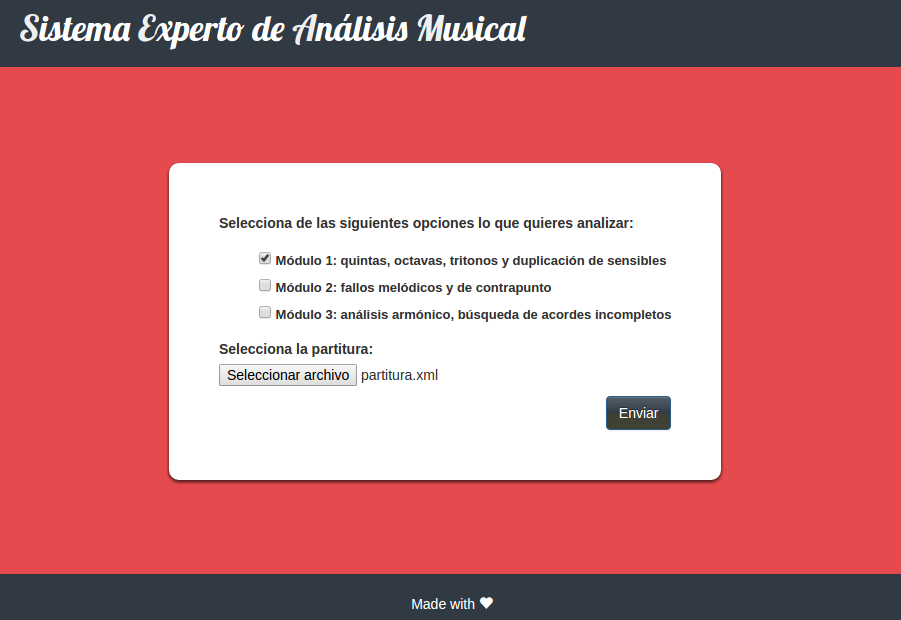
\includegraphics[scale=0.35]{imagenes/interfaz3.png}
	\caption{Página principal}
	\label{fig5.3.1}
\end{figure}

\begin{figure}[H]
	\centering
	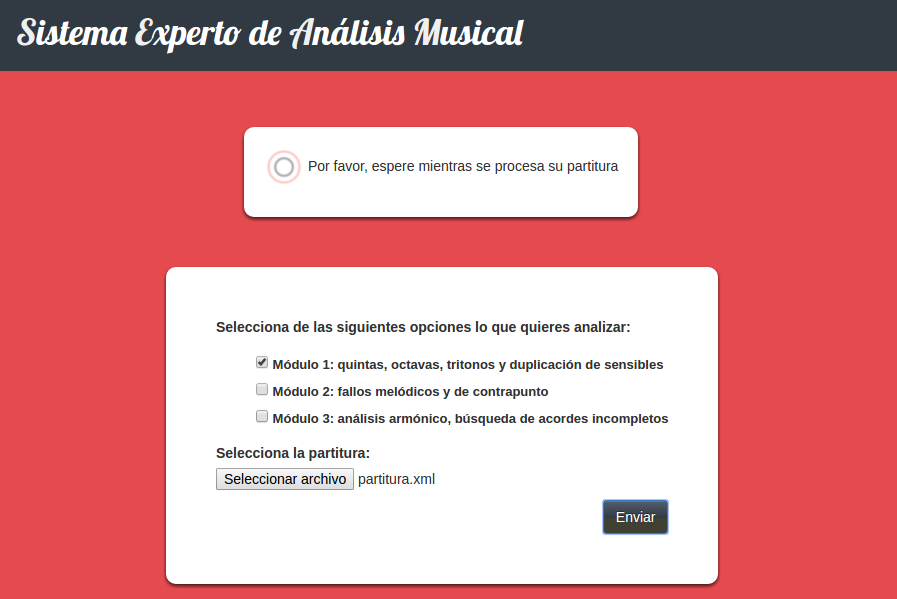
\includegraphics[scale=0.35]{imagenes/interfaz4.png}
	\caption{Página principal tras enviar el formulario}
	\label{fig5.3.2}
\end{figure}

\bigskip

\begin{figure}[H]
	\centering
	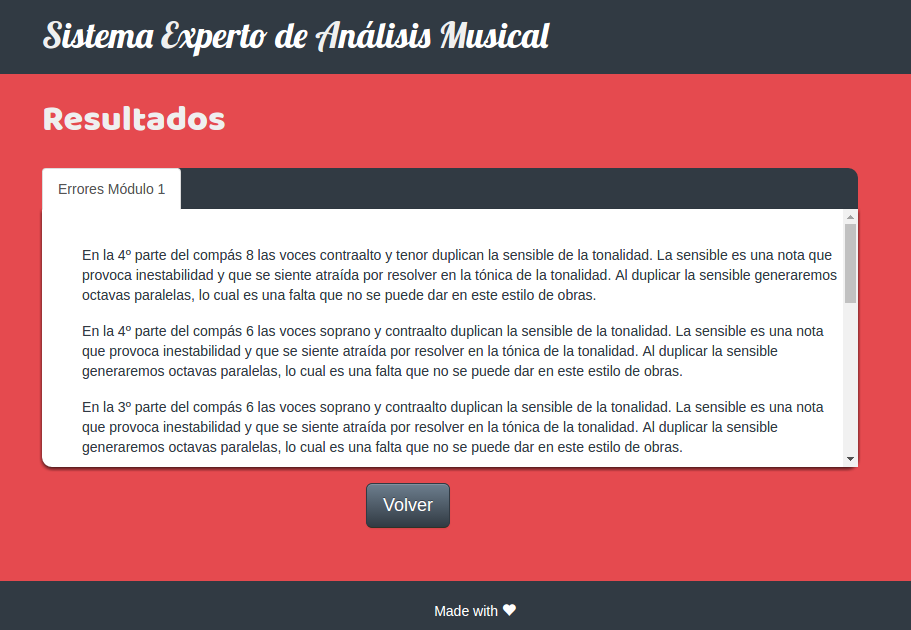
\includegraphics[scale=0.35]{imagenes/interfaz5.png}
	\caption{Visualización de resultados con errores}
	\label{fig5.3.3}
\end{figure}

\begin{figure}[H]
	\centering
	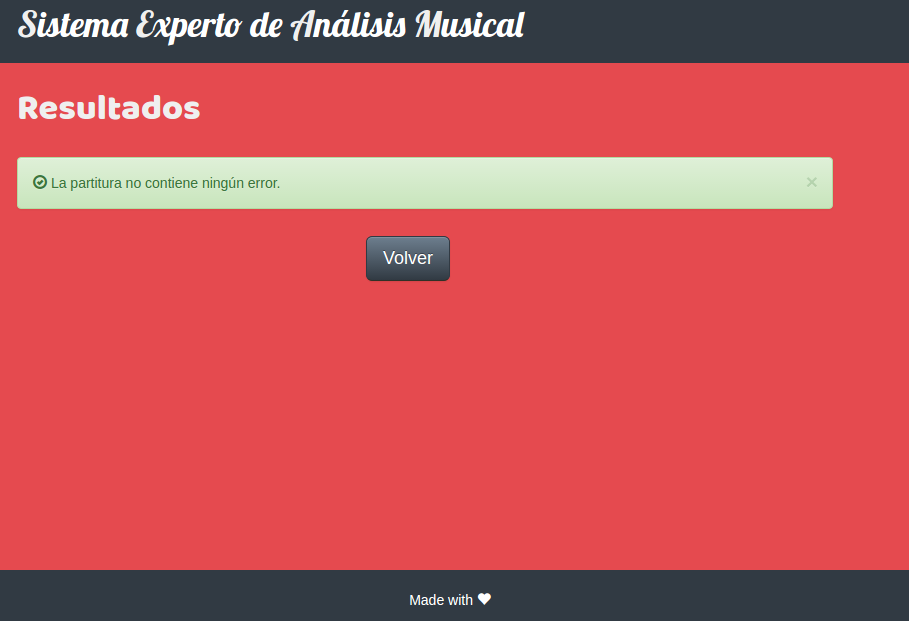
\includegraphics[scale=0.35]{imagenes/interfaz6.png}
	\caption{Visualización de resultados sin errores}
	\label{fig5.3.4}
\end{figure}
%\chapter{Pruebas y validación}

Con toda la implementación del sistema realizada, pasamos a la fase de verificación y validación del sistema. 

\section{Verificación}

Como describimos en el capítulo anterior, la verificación del sistema experto consistió en comprobar que accedía y leía bien el contenido de los ficheros y añadía los hechos a la memoria de trabajo de manera correcta. 

Como no podíamos comprobarlo visualmente como hicimos con el prototipo, se hicieron pruebas en las que el sistema experto, además de los errores, mostraba los hechos asertados, hechos calculados y hechos leídos. 

Una vez se comprobó que el sistema experto se ejecutaba correctamente, pasamos a comprobar las funcionalidades de la interfaz.

Primero se comprobó que las funciones de extracción de información del archivo XML obtenían y guardaban correctamente los datos. Para ello, se ejecutaron todas las funciones con distintas partituras y se revisaron los ficheros resultantes para ver si coincidían con el formato escogido y no contenían fallos.

También se verificó el funcionamiento del envío del formulario para que no se produjesen las siguientes situaciones:

\begin{itemize}

	\item No se puede enviar un formulario en blanco.
	\item No se puede enviar un archivo sin seleccionar ninguna opción.
	\item No se puede enviar la lista de opciones sin adjuntar un archivo.
	\item El archivo a adjuntar debe ser de formato XML.

\end{itemize}

Por último, se examinó que los resultados se mostrasen de manera legible y ordenados en sus pestañas correspondientes. Las pestañas de los módulos deben mostrarse si se ha seleccionado dicho módulo y si se han obtenido errores. En caso contrario, no deberían de mostrarse.

\section{Validación}

La validación del sistema experto fue llevada a cabo por Clara Luz Fernández Vecino, profesora de armonía del Conservatorio Ángel Barrios de Granada.

Para ello, el sistema analizó ejercicios realizados por los alumnos del conservatorio:

\begin{itemize}

	\item Alrededor de 100 ejercicios de armonía. Con estos ejercicios se validaron los módulos de errores provocados por los movimientos y algunos errores armónicos. 

	\item 20 ejercicios de composición de corales. Con estas composiciones se validaron todos los módulos, especialmente el módulo de análisis melódico.

\end{itemize}

Tras ejecutar el sistema, Clara Luz revisó los resultados obtenidos por el sistema comparándolos con las correcciones que ella misma había llevado a cabo sobre todos los ejercicios.
%\chapter{Resultados y conclusiones}

\section{Resultados}

Los resultados obtenidos tras la validación del sistema por Clara Luz han sido entre un 85-90\% de acierto. Esto significa que de todos los errores señalados por Clara Luz, el sistema detecto el 85-90\% de todos ellos aproximadamente.

En los casos de errores no detectados, se debía a que eran situaciones extremas o excepcionales que no había considerado para el desarrollo del sistema, como por ejemplo resoluciones excepcionales de séptimas o detección de quintas paralelas entre acordes sin tener en cuenta las notas de paso. 

Sin embargo, el sistema en muchos de los ejemplos, fue capaz de detectar errores que no habían sido encontrados por Clara Luz. Esta cantidad de errores podían ser desde encontrar un error no señalizado a incluso diez o más, por lo que es difícil estimar un porcentaje claro.

Si no tenemos en cuenta el porcentaje de error debido a casos no contemplados por el sistema o no implementados, el sistema encuentra prácticamente todos los errores, suponiendo un 95\% o más de acierto.

\bigskip

Respecto al tiempo empleado para analizar las partituras, si comparamos el tiempo empleado por el sistema con la interfaz web y sin ella, los resultados no son muy favorables. La ejecución del sistema experto en el entorno de CLIPS tarda unos pocos segundos, mientras que con la interfaz tarda entre 1 y 5 minutos. 

\section{Conclusiones}

En relación a los resultados referidos al porcentaje de errores encontrados, considero que dada la complejidad de la tarea, se han obtenido buenos resultados. 

He de destacar el hecho de que el sistema encontró errores que no habían sido señalados por Clara Luz. Esto supone que el sistema, en algunas ocasiones, puede analizar partituras mejor o con más detalle que un experto. Obviamente en el caso del experto siempre está el factor humano y la garantía de cometer errores más fácilmente que una máquina. Aún así, este hecho fue una muy grata sorpresa.

También destacar el hecho de que si en la partitura se encuentra alguno de los errores o faltas que se describen en los requisitos, siempre es capaz de detectarlos y señalarlos, lo cual satisface por completo los objetivos propuestos.

\bigskip
En cuanto a los resultados sobre el tiempo de ejecución, el hecho de crear la interfaz web ha supuesto una pérdida de velocidad considerable. 

Al haber embebido el sistema dentro de una aplicación web, se ha perdido una de las mejores características de CLIPS, que es su velocidad de procesamiento. Esta ventaja de CLIPS se ha sacrificado para poder hacer un sistema más accesible y con una interfaz más afable, dado que es muy improbable que los usuarios finales tengan algún conocimiento sobre CLIPS o su existencia. 

Por otro lado, para un experto, estos análisis tan exhaustivos pueden llevar alrededor de 20 minutos para un coral de 24-32 compases, que suele ser la longitud media de este tipo de obras. Teniendo en cuenta esta comparación, el sistema tarda, como mínimo, cuatro veces menos que un experto, lo cual supone una ganancia en tiempo bastante aceptable.

Dado que el tiempo no era realmente un requisito indispensable o un objetivo propuesto no le he dado demasiada importancia a la pérdida de eficiencia que nos ha supuesto la interfaz, y más si tenemos en cuenta que para el usuario supone una mejora respecto a hacer el análisis manualmente. 

Aún así he realizado algunas pruebas y mediciones sobre la ejecución del sistema con la interfaz. He podido comprobar que la pérdida de velocidad no radica en la ejecución del sistema experto sino que parece estar más bien relacionada con procesar los resultados para poder mostrarlos de manera correcta. Esto significa que el problema no está relacionado con la implementación del sistema experto sino con alguno de los procedimientos que se llevan a cabo en la interfaz o con su conexión entre el servidor y el usuario.

\bigskip

Teniendo en cuenta todo lo anterior, podemos concluir que este sistema proporciona unos resultados bastante buenos en un tiempo bastante aceptable y que hemos podido satisfacer todos los requisitos y alcanzar los objetivos propuestos.

\section{Futuro desarrollo}

Uno de los motivos principales por los que se escogió hacer un sistema experto es por su gran escalabilidad. Este proyecto puede ser ampliado en una gran cantidad formas:

\begin{itemize}

	\item Añadiendo nuevas reglas de armonía y/o excepciones a los módulos de análisis ya existentes.
	\item Añadiendo nuevos módulos para analizar otros aspectos o estilos musicales.
	\item Adaptando los módulos a otros tipos de obras y formas musicales, como obras para piano, orquesta, ...
	\item Añadir nuevas funcionalidades a la aplicación como creación de usuarios, llevar un registro de las partituras analizadas, añadir estadísticas, ...
\end{itemize}

\bigskip

Además, está el hecho de que se puede intentar mejorar la eficiencia del sistema utilizando programación concurrente, mejorando el uso de la memoria o incluso intentar trasladarlo a otro tipo de interfaz que pueda ser más eficiente en términos de velocidad.

\bigskip
En definitiva, este sistema aún tiene muchas posibilidades de mejorar y crecer, aunque como primera versión ha dado unos resultados más que satisfactorios.

%----------------------------------------------------------------------------------------
%	Glosario
%----------------------------------------------------------------------------------------


%----------------------------------------------------------------------------------------
%	Referencias
%----------------------------------------------------------------------------------------

\bibliography{bibliografia} %archivo bibliografia.bib que contiene las entradas 
\bibliographystyle{plain} 

\end{document}